% --------------------------------------------------------------------------- %
% Poster for the ECCS 2011 Conference about Elementary Dynamic Networks.      %
% --------------------------------------------------------------------------- %
% Created with Brian Amberg's LaTeX Poster Template. Please refer for the     %
% attached README.md file for the details how to compile with `pdflatex`.     %
% --------------------------------------------------------------------------- %
% $LastChangedDate:: 2011-09-11 10:57:12 +0200 (V, 11 szept. 2011)          $ %
% $LastChangedRevision:: 128                                                $ %
% $LastChangedBy:: rlegendi                                                 $ %
% $Id:: poster.tex 128 2011-09-11 08:57:12Z rlegendi                        $ %
% --------------------------------------------------------------------------- %
\documentclass[a0paper,portrait]{baposter}
\usepackage{gensymb}
\usepackage{amssymb}
\usepackage{relsize}		% For \smaller
\usepackage{url}			% For \url
\usepackage{epstopdf}	% Included EPS files automatically converted to PDF to include with pdflatex

%%% Global Settings %%%%%%%%%%%%%%%%%%%%%%%%%%%%%%%%%%%%%%%%%%%%%%%%%%%%%%%%%%%

\graphicspath{{pix/}}	% Root directory of the pictures 
\tracingstats=2			% Enabled LaTeX logging with conditionals

%%% Color Definitions %%%%%%%%%%%%%%%%%%%%%%%%%%%%%%%%%%%%%%%%%%%%%%%%%%%%%%%%%

\definecolor{bordercol}{RGB}{40,40,40}
\definecolor{headercol1}{RGB}{186,215,230}
\definecolor{headercol2}{RGB}{80,80,80}
\definecolor{headerfontcol}{RGB}{0,0,0}
\definecolor{boxcolor}{RGB}{186,215,230}

%%%%%%%%%%%%%%%%%%%%%%%%%%%%%%%%%%%%%%%%%%%%%%%%%%%%%%%%%%%%%%%%%%%%%%%%%%%%%%%%
%%% Utility functions %%%%%%%%%%%%%%%%%%%%%%%%%%%%%%%%%%%%%%%%%%%%%%%%%%%%%%%%%%

%%% Save space in lists. Use this after the opening of the list %%%%%%%%%%%%%%%%
\newcommand{\compresslist}{
	\setlength{\itemsep}{1pt}
	\setlength{\parskip}{0pt}
	\setlength{\parsep}{0pt}
}

%%%%%%%%%%%%%%%%%%%%%%%%%%%%%%%%%%%%%%%%%%%%%%%%%%%%%%%%%%%%%%%%%%%%%%%%%%%%%%%
%%% Document Start %%%%%%%%%%%%%%%%%%%%%%%%%%%%%%%%%%%%%%%%%%%%%%%%%%%%%%%%%%%%
%%%%%%%%%%%%%%%%%%%%%%%%%%%%%%%%%%%%%%%%%%%%%%%%%%%%%%%%%%%%%%%%%%%%%%%%%%%%%%%

\begin{document}
\typeout{Poster rendering started}

%%% Setting Background Image %%%%%%%%%%%%%%%%%%%%%%%%%%%%%%%%%%%%%%%%%%%%%%%%%%
\background{
	\begin{tikzpicture}[remember picture,overlay]%
	\draw (current page.north west)+(-2em,2em) node[anchor=north west]
	{
\includegraphics[height=1.1\textheight]{background}};
	\end{tikzpicture}
}

%%% General Poster Settings %%%%%%%%%%%%%%%%%%%%%%%%%%%%%%%%%%%%%%%%%%%%%%%%%%%
%%%%%% Eye Catcher, Title, Authors and University Images %%%%%%%%%%%%%%%%%%%%%%
\begin{poster}{
	grid=false,
	% Option is left on true though the eyecatcher is not used. The reason is
	% that we have a bit nicer looking title and author formatting in the headercol
	% this way
	%eyecatcher=false, 
	borderColor=bordercol,
	headerColorOne=headercol1,
	headerColorTwo=headercol2,
	headerFontColor=headerfontcol,
	% Only simple background color used, no shading, so boxColorTwo isn't necessary
	boxColorOne=boxcolor,
	headershape=roundedright,
	headerfont=\Large\sf\bf,
	textborder=rectangle,
	background=user,
	headerborder=open,
  boxshade=plain
}
%%% Eye Cacther %%%%%%%%%%%%%%%%%%%%%%%%%%%%%%%%%%%%%%%%%%%%%%%%%%%%%%%%%%%%%%%
{
	Eye Catcher, empty if option eyecatcher=false - unused
}
%%% Title %%%%%%%%%%%%%%%%%%%%%%%%%%%%%%%%%%%%%%%%%%%%%%%%%%%%%%%%%%%%%%%%%%%%%
{\sf\bf
	Observations of PKiKP and Precursors to ScS
}
%%% Authors %%%%%%%%%%%%%%%%%%%%%%%%%%%%%%%%%%%%%%%%%%%%%%%%%%%%%%%%%%%%%%%%%%%
{
	\vspace{1em} Long Xin${}^{1}$, Hitoshi Kawakatsu${}^{2}$\\
	{\normalsize ${}^{1}$Institute of Geology and Geophysics, Chinese Academy of Sciences%
\\${}^{2}$Earthquake Research Institute, University of Tokyo}
}
%%% Logo %%%%%%%%%%%%%%%%%%%%%%%%%%%%%%%%%%%%%%%%%%%%%%%%%%%%%%%%%%%%%%%%%%%%%%
{
% The logos are compressed a bit into a simple box to make them smaller on the result
% (Wasn't able to find any bigger of them.)
\setlength\fboxsep{0pt}
\setlength\fboxrule{0pt}
	\fbox{
		\begin{minipage}{9em}
			\centering
			\includegraphics[width=8em,height=8em]{cas_logo}
		\end{minipage}
	}
}

\headerbox{Introduction}{name=intro,row=0,column=0}{%
$\blacksquare$The properties of inner and outer core boundary, ICB, which is a thermal, physical and chemical boundary is important for us to know the evolution history of the earth. The seismic phase PKiKP, which reflected from ICB, can bring information about this boundary such as density jump, topography, and possible regional variation of them. However, it's rare to be seen compared to other core phases like PKIKP because of the smaller reflection coefficient\cite{Shearer1990}. 

$\blacksquare$ScSp, P wave converted from ScS on the subsurface in the mantle is a evidence of subducting slab, and the observation of this phase in Japan islands has been reported by several authors\cite{Nakanishi1980}. by using this phase, one can estimate the depth of slab and its seismic properties, and it also provides chance to examine the continuation of subducting plates.
}

\headerbox{Global PKiKP Observations}{name=pkikp,column=0,below=intro}{%

\includegraphics[width=\linewidth]{global.eps}
Using small arrays of International Monitor System(IMS), Observed PKiKP data for 265 array and event pairs are collected.
\vspace{-0.5em}
\begin{center}
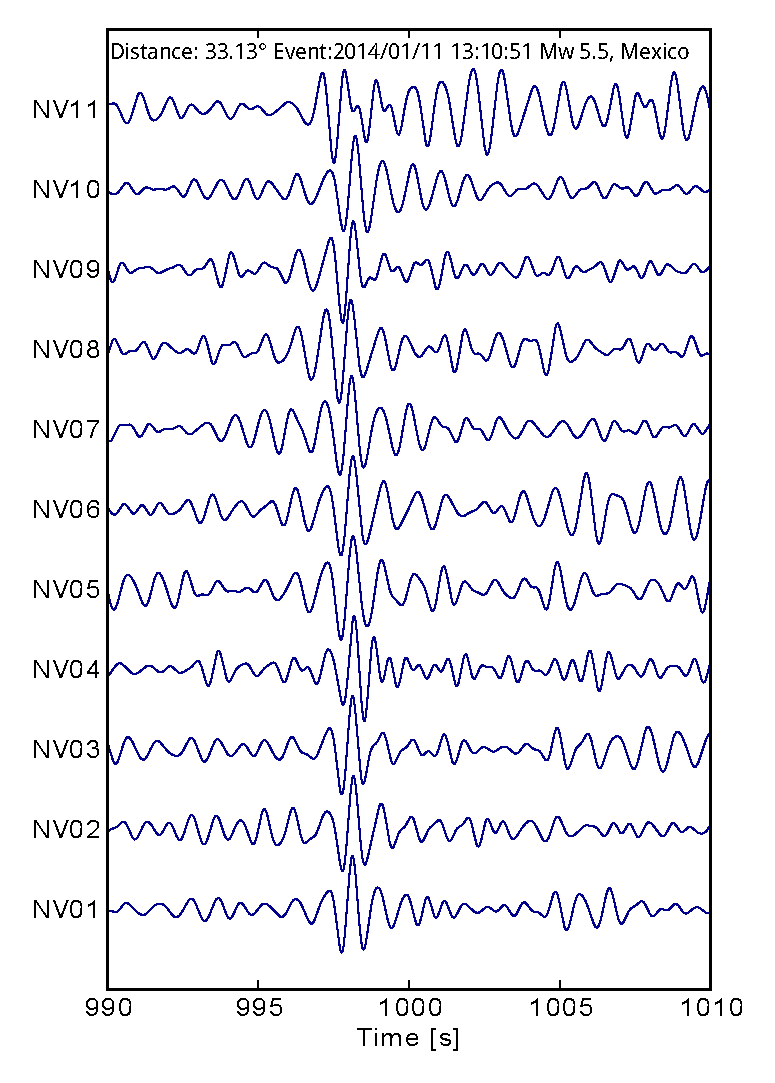
\includegraphics[width=0.85\linewidth]{pkikp_nvar.eps}
\end{center}
\vspace{-0.5em}
In those data, there many observations of high quality, where waveforms of PKiKP are very clear and can be seen in all the traces of the array. Above figure is PKiKP observed in NVAR. Those PKiKP signals are also similar to PcP in this observation, which may give convincing amplitude measurements.
}

\headerbox{Reference}{name=ref,column=0,below=pkikp,above=bottom,span=2}{%
\smaller
\vspace{-0.4em}
\bibliographystyle{plain}
\renewcommand{\section}[2]{\vskip 0.05em}
\bibliography{sub,innercore}
}

\headerbox{PKiKP/PcP Amplitude Ratio}{name=amp,column=1,row=0}{%
When the distance is short, ray path of PcP and PKiKP in the mantle can be considered to be close, so mantel effect may be partly cancled.
\begin{center}
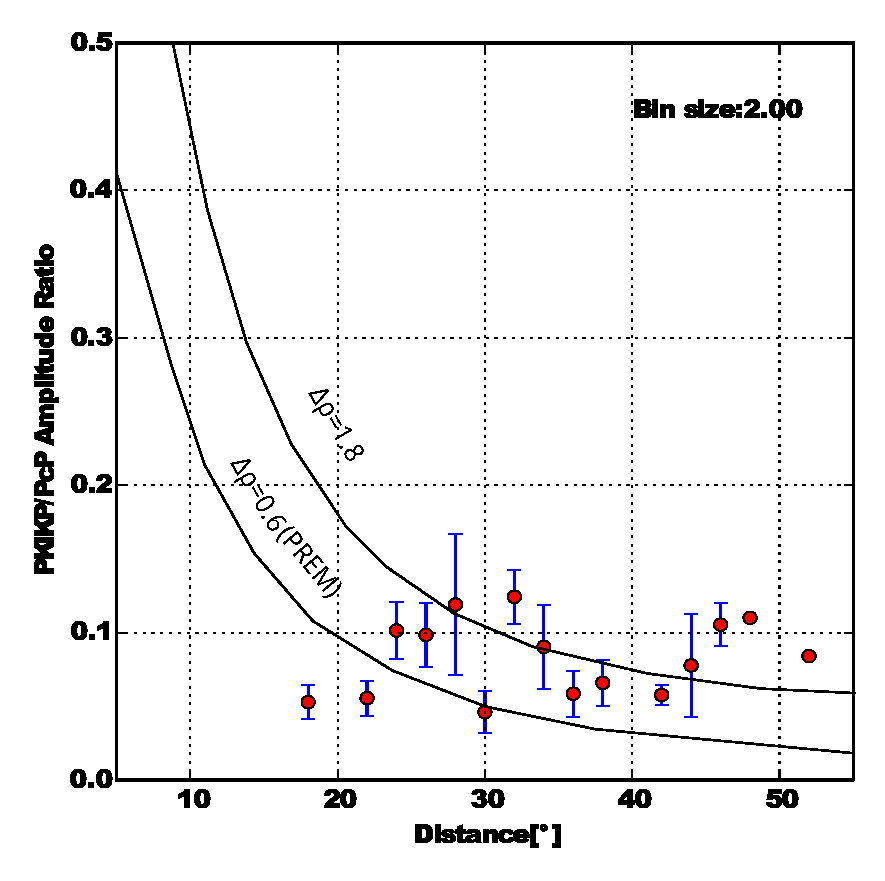
\includegraphics[width=0.8\linewidth,height=0.8\linewidth]{amp.eps}
\end{center}
\vspace{-1em}
Assuming the parameter of CMB  be known and heterogeneity of the lower mantle should not be strong, the result may indicate the density jump of ICB is larger than that given by PREM. 
}

\headerbox{ScSp Observations in Japan Islands}{name=scsp,column=1,span=2,below=amp}{%

\begin{minipage}{0.4\linewidth}
Because of the S to P conversion, ScSp arrives earlier than ScS, and its amplitude is much smaller than ScS. Right is a example of ScSp observation on F-Net station KISF, it could be seen that ScSp is about 4s earlier than ScS. ScS is strongest in North-East component and ScSp only is visible on the vertical component, which coincides with westward subducting of the slab.
\end{minipage}
\hfil{}
\begin{minipage}{0.58\linewidth}
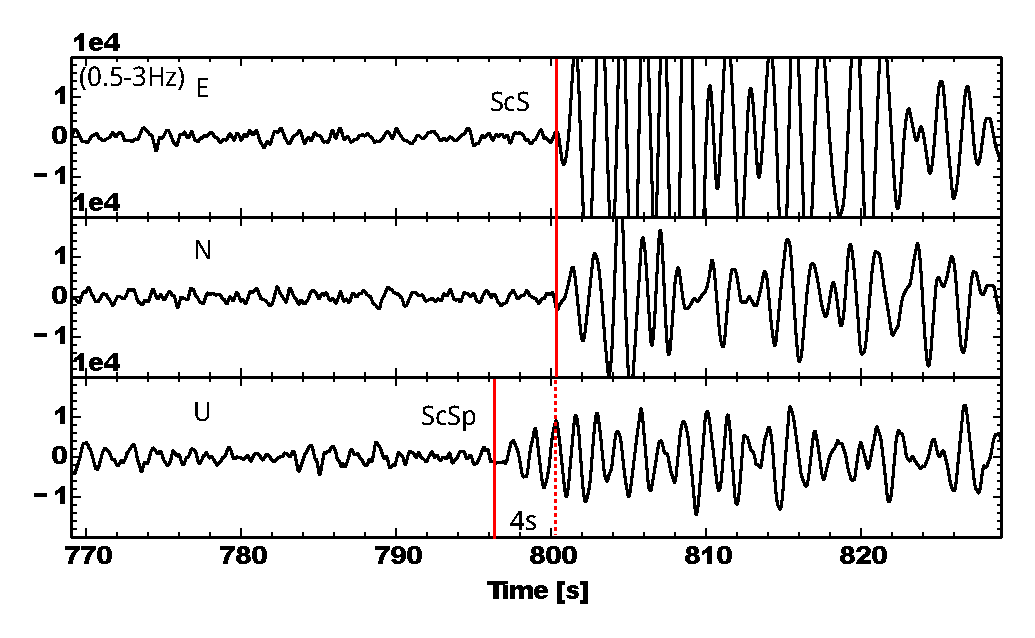
\includegraphics[width=\linewidth,height=0.45\linewidth]{mul.eps}
\end{minipage}
}

\headerbox{Slab Depth Beneath Stations}{name=slab,column=1,below=scsp,above=ref}{%
\includegraphics[width=\linewidth]{slab1.eps}
North-westward subducting Philippine plate and eastward subducting Pacific plate intersect in the south-west of Japan. The locations of white circles coincide with stations, and the size of them stands for time difference between ScS and ScSp for a deep event(2015/05/30,Mw 7.8,680 km,Bonin Islands). Almost all ScSp observations are in South-West of Japan, and time difference indicate a average slab depth of 50km as described by previous authors\cite{Nakanishi1980,Nakanishi1981}. 
}

\headerbox{Diff Travel Time Residual}{name=time,column=2,row=0,above=scsp}{%
\vspace{-1.5em}
\[ T_{res} = (T_{PKiKP}^{obs} - T_{PcP}^{obs}) - (T_{PKiKP}^{prem} - T_{PcP}^{prem}) \]
\begin{center}
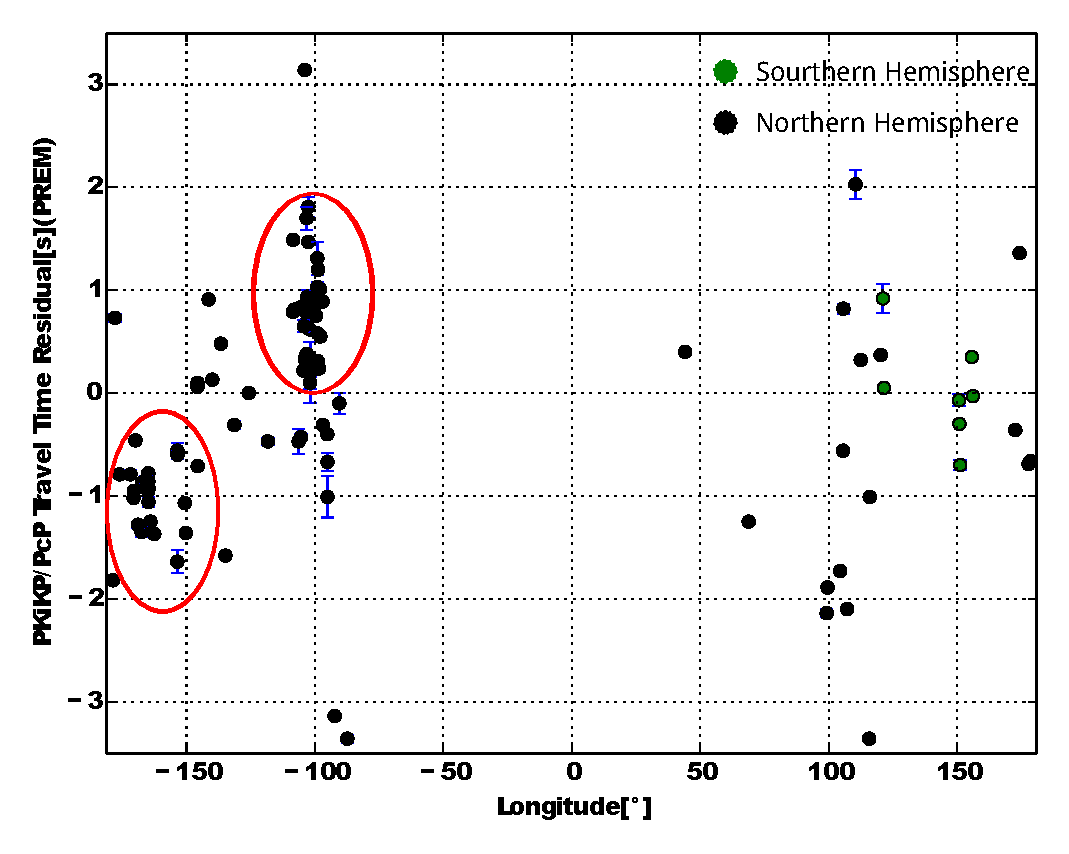
\includegraphics[width=0.9\linewidth]{time_res.eps}
\end{center}
\vspace{-0.5em}
Figure above shows PcP and PKiKP difference time residual calculated using PREM model ploted against longitude of ICB bounce points of PKiKP. It seems that clear variation exists between two sides of 150$\degree$W, which indicates that probable variation of ICB topography is about 10km. 
}

\headerbox{Location of Conversion Point}{name=mod,column=2,below=scsp,above=bottom}{%
\begin{center}
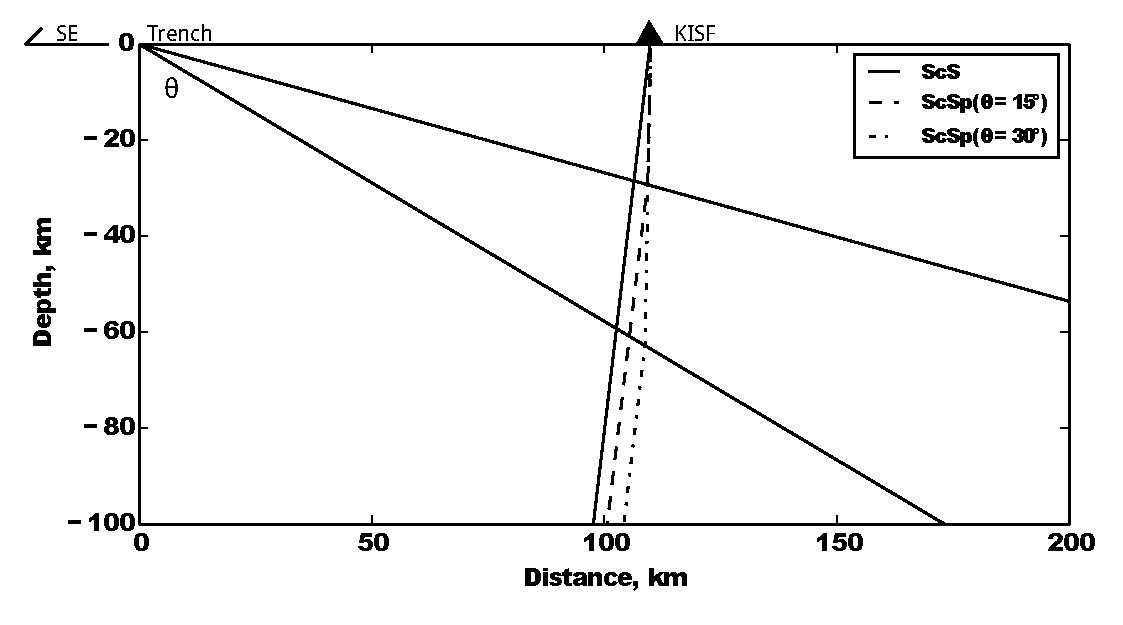
\includegraphics[width=0.9\linewidth]{ray_path.eps}
\end{center}
\vspace{-0.8em}
Differential time $\tau_{ScS-ScSp}$ is determined by the depth of slab beneath
the station. By using ray tracing, the location of the S to P conversion point
can be decided, so the depth of the slab can be inferred.
\vspace{-0.4em}
\begin{center}
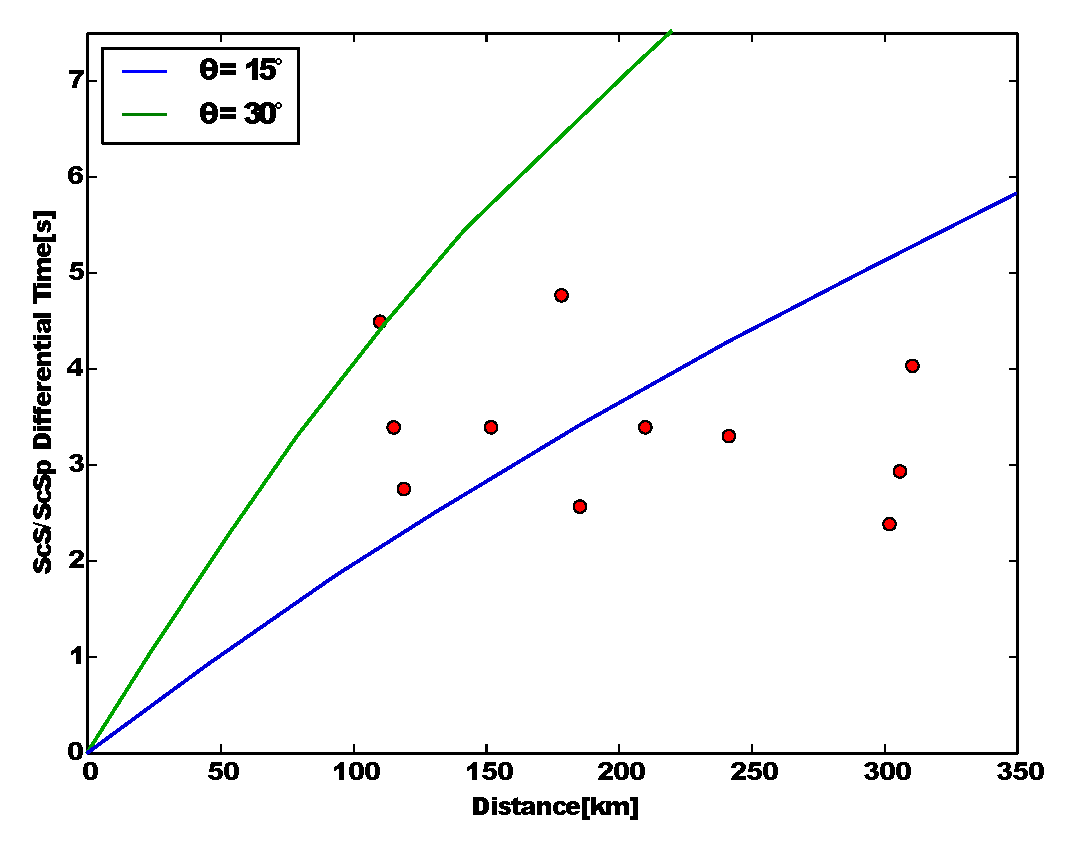
\includegraphics[width=0.9\linewidth,height=0.65\linewidth]{diff_time.eps}
\end{center}
\vspace{-0.5em}
Theoretical $\tau_{ScS-ScSp}$ are plotted against distance from trench for dipping angle of the slab $15\degree$ and $30\degree$ respectively, observations above Ryukyu slab are also plotted as red points. The result may indicates that the slab is quite flat beneath south-east region of Japan.
}

\end{poster}
\end{document}

